\documentclass[a4paper,12pt]{article}

%\usepackage{amsmath,amssymb,multicol,tikz,enumitem}
\usepackage[margin=2cm]{geometry}
%\usetikzlibrary{calc}
\usepackage{amsmath}
\usepackage{amsthm}
\usepackage{amssymb}
\usepackage{thmtools}
\usepackage{hyperref}
\usepackage{enumerate}
\usepackage{graphicx}
\usepackage{xcolor}

\pagestyle{empty}

\newcommand\Q{\mathbf{Q}}
\newcommand\R{\mathbf{R}}
\newcommand\Z{\mathbf{Z}}

\usepackage{array}
\newcolumntype{P}[1]{>{\centering\arraybackslash}p{#1}}

\newcommand\indd{${}$\hspace{20pt}}

\declaretheoremstyle[headfont=\normalfont\bfseries,notefont=\mdseries\bfseries,bodyfont = \normalfont,headpunct={:}]{normalhead}
\declaretheorem[name={Uzdevums}, style=normalhead,numberwithin=section]{problem}

\setcounter{section}{1}

\setlength\parindent{0pt}

\begin{document}

\begin{center}
\parbox{3.5cm}{\flushleft\bf Skaitļu teorija\linebreak NMS juniori} \hfill {\bf \large Mājasdarba \#1 atrisinājumi} \hfill \parbox{3.5cm}{\flushright\bf 2020./2021.m.g.} \\[2pt]
\rm\small 2020.gada 10.oktobris
\end{center}

%\hrule\vspace{2pt}\hrule
\hrule

\vspace{20pt}
{\bf Iesniegšanas termiņš:} 2020.g.\ 31.oktobris\\
{\bf Kam iesūtīt:} {\tt kalvis.apsitis}, domēns {\tt gmail.com}


\vspace{20pt}
{\bf Uzdevums 1.1:} 
Dota kopa $S = \{ 105,106,\ldots,210 \}$. Noteikt mazāko
naturālo $n$ vērtību, ka, izvēloties jebkuru $n$ skaitļu
apakškopu $T$ no kopas $S$, tajā būs vismaz divi skaitļi, kuri nav
savstarpēji pirmskaitļi.


\vspace{20pt}
{\bf Uzdevums 1.2:}
Visiem naturāliem skaitļiem $m > n$ pierādīt, ka
$$\mbox{MKD}(m,n) + \mbox{MKD}(m+1,n+1) > \frac{2mn}{\sqrt{m-n}}.$$
(Ar $\operatorname{MKD}(a,b)$ apzīmē naturālu skaitļu $a$ un $b$ {\em mazāko 
kopīgo dalāmo} \textendash{} mazāko skaitli, kas dalās gan ar $a$, gan ar $b$.)


\vspace{20pt}
{\bf Uzdevums 1.3:}
Vai eksistē bezgalīga
stingri augoša naturālu skaitļu virkne $a_1 < a_2 < a_3 <\ldots$,
ka jebkuram fiksētam naturālam skaitlim $a$ virknē 
$$a_1+a < a_2+a < a_3 + a < \ldots$$
ir ne vairāk kā galīgs skaits pirmskaitļu?

\vspace{20pt}
{\bf Uzdevums 1.4:}
Pierādīt, ka virkne $1,11,111,\ldots$ satur bezgalīgu apakšvirkni,
kuras katri divi locekļi ir savstarpēji pirmskaitļi.



\vspace{20pt}
{\bf Uzdevums 1.5:}
Pierādīt vai apgāzt sekojošus apgalvojumus:
\begin{enumerate}[(A)]
\item Jebkuram $k \geq 2$, un jebkuriem $k$ pēc kārtas sekojošiem naturāliem 
skaitļiem starp tiem varēs atrast skaitli, kurš nedalās ne ar vienu pirmskaitli, kas mazāks par $k$.   
\item Jebkuram $k \geq 2$, un jebkurai $k$ pēc kārtas sekojošu naturālu skaitļu virknei starp virknes locekļiem varēs atrast skaitli, 
kas ir savstarpējs pirmskaitlis ar visiem citiem virknes locekļiem. 
\end{enumerate}

\newpage

{\bf Ieteikumi un teorija: Pārdomas pirms atrisinājumiem}

\vspace{5pt}
Daži ieteikumi ir vispārīgas metodes ({\bf trekniem burtiem}), ko labi prast lietot, jo tās der daudziem uzdevumiem. 
Teorijas tēmas arī var palīdzēt, bet nereti bez tām var iztikt. Radošums, risinājuma metodes elastība
ļauj lietot to teoriju, kuru olimpiādē atceramies.


{\footnotesize
\vspace{5pt}
{\bf Uzdevums 1.1:} 
\begin{enumerate}
\item {\bf Nosacījuma ``tulkošana'':} Vai var izteikt frāzi {\em ``vismaz divi skaitļi, kuri nav savstarpēji pirmskaitļi''} kaut kā citādi? 
\item {\bf Vienkāršot sev dzīvi:} Vai var pamatot līdzīgu apgalvojumu (mazākiem skaitļiem)? Vispārīgāku apgalvojumu? 
\item {\bf Sākšana no beigām:} Iedomāsimies, ka esam jau atrisinājuši (atraduši mazāko $n$). Vai var par šo $n$ pateikt pretēju (vieglāk saprotamu? konstruktīvāku) apgalvojumu?
\item Teorija: Skaitļa dalījums pirmreizinātājos (aritmētikas pamatteorēma).
%(sk. \url{https://bit.ly/3eht2a3}). 
Pirmskaitļu pārbaude ar pilno pārlasi (skaitli $n$ dala ar $2,3,\ldots,\sqrt{n}$. 
%sk. \url{https://bit.ly/2JoqvQ9}). 
Dirihlē princips.
%(sk. \url{https://bit.ly/31ZlQKY}).
\end{enumerate}


{\bf Uzdevums 1.2:} 
\begin{enumerate}
\item {\bf Nosacījumu pārbaude:} Vai apgalvojumā esošo nevienādību var kaut kā ``sasniegt'' vai tai 
``pietuvoties''; kādiem skaitļu pāriem tas izdodas? 
\item {\bf Sākšana no beigām:} Ja pierādāmajā nevienādībā ietilpst kvadrātsakne, kā izskatās
mums zināmas citas nevienādības ar kvadrātsakni un kā līdz tai nonākts šajās situācijās.
\item Teorija: Nevienādību pierādīšana, veidojot nevienādību ķēdīti (pēdējo nevienādību ķēdītē mākam pierādīt, un no tās seko 
visas iepriekšējās). Identitāte, kas saista LKD un MKD: $\mbox{LKD}(a,b) \cdot \mbox{MKD}(a,b) = ab$.\\
Nevienādība par vidējo aritmētisko un vidējo ģeometrisko: ${\displaystyle \frac{a+b}{2} \geq \sqrt{ab}}$.\\
Divi pēc kārtas sekojoši skaitļi ir savstarpēji pirmskaitļi: $\mbox{LKD}(a,a+1)=1$.\\
Eiklīda algoritms LKD atrašanai. 
\end{enumerate}


{\bf Uzdevums 1.3:} 
\begin{enumerate}
\item {\bf Vizualizācija:} Vai virknītes, kas jāaplūko uzdevumā var attēlot, piemēram divās dimensijās (kā plaknes punktus vai rūtiņas)?
\item Teorija: Eksistē cik patīk garas pēc kārtas sekojošas skaitļu virknes bez pirmskaitļiem.\\
(Piemēram, $(n+1)!+2,\ldots,(n+1)!+(n+1)$ ir 
$n$ pēc kārtas sekojoši salikti skaitļi.)\\
%(sk. rezultātus par pirmskaitļu atstarpēm/{\em gaps}: \url{https://bit.ly/2HNLo6D}). 
No dažām neveiksmīgām konstrukcijām mūs var pasargāt Dirihlē teorēma par pirmskaitļu skaitu arit\-mē\-tis\-kās progresijās (Vai nu 
aritmētiskā progresijā pirmskaitļu ir bezgalīgi daudz, vai arī to ir ne vairāk kā viens \textendash{} 
gadījumos, kad progresijas pirmais loceklis un diference nav savstarpēji pirmskaitļi).
Šī teorēma ir grūti pierādāma (un tā, protams, nav jāzina un jāizmanto).
%(sk. \url{https://bit.ly/35M1Nka}).
\end{enumerate}


{\bf Uzdevums 1.4:} 
\begin{enumerate}
\item {\bf Ķēpāšanās/Eksperimentēšana:} Kā uzrakstīt vismaz dažus pirmos virknes locekļus, kuri ir savstarpēji pirmskaitļi? 
\item Teorija: Eiklīda algoritms LKD atrašanai.
%(sk.\ \url{https://bit.ly/3oLalR6})
Dalīšana stabiņā.
%(sk. \url{https://bit.ly/37Ydd7h}). 
Ģeometriskas progresijas summa.
%(sk. \url{https://bit.ly/35OakmN}). 
\end{enumerate}


{\bf Uzdevums 1.5.A:} 
\begin{enumerate}
\item {\bf Pretējais apgalvojums:} Kā noformulēt šajā punktā paustā apgalvojuma noliegumu?
\item {\bf Ķēpāšanās/Eksperimentēšana:} Vai var izmēģināt dažas nelielas $k$ vērtības? 
\item Teorija: Gadījumu pārlase.
%(sk. \url{https://bit.ly/3mL666l}). 
\end{enumerate}


{\bf Uzdevums 1.5.B:} 
\begin{enumerate}
\item {\bf Ķēpāšanās/Eksperimentēšana:} Vai var izmēģināt dažas nelielas $k$ vērtības?
\item {\bf Meklējumu telpas samazināšana:} Ja meklējam pretpiemēru, kuras $k$ vērtības ir vērts aplūkot? (Nē, tās nav visas naturālās; 
daudzas $k$ vērtības var mierīgi izlaist, neko interesantu nezaudējot.)
\item {\bf Vizualizācija:} Kā skaitļu virknītes zīmējumā uzskatāmi attēlot, ka diviem skaitļiem ir kopīgs dalītājs.
\item Teorija: Gadījumu pārlase.
% (sk. \url{https://bit.ly/3mL666l}). 
Eratostēna režģis.
% (sk. \url{https://bit.ly/3oJDlZl}).
\end{enumerate}

}



\newpage

{\bf Uzdevums 1.1:} Atbilde $n = 26$.\\
Risināsim vispirms ``pretējo'' uzdevumu \textendash{} kā atrast lielāko apakškopu $A$,
kurā katri divi elementi $a_1,a_2 \in A$ ir savstarpēji pirmskaitļi. 

{\bf Definīcija.} Sauksim veselu skaitļu kopu $A \subseteq [105;210]$ par {\em maksimālu}, 
ja tajā katri divi elementi ir savstarpēji pirmskaitļi un tās elementu skaits $|A|$ ir lielākais iespējamais.

{\bf Apgalvojums 1.} Visi pirmskaitļi no intervāla $[105,210]$ noteikti pieder maksimālai kopai $A$.\\
{\em Pierādījums.} Jebkuram pirmskaitlim ($107$,$109$ utt.) neviens daudzkārtnis (divkāršojums, trīskāršojums, utt.) 
nebūs intervālā $[105;210]$. Tātad šie pirmskaitļi ar citiem skaitļiem $[105;210]$ nekonfliktē; ja tos nepievienotu, 
kopas $A$ elementu skaits vairs nebūtu maksimālais. Šos pirmskaitļus var atrast ar Eratostēna režģi vai, 
pārbaudot dalāmību:
$$\{ 107, 109, 113, 127, 131, 137, 139, 149, 151, 157, 163, 167, 173, 179, 181, 191, 193, 197, 199\}.\;\;\blacksquare$$

{\bf Apgalvojums 2.} Eksistē tāda maksimāla kopa $A$, kurā ir pirmskaitļu pakāpes $a_2 = 2^7 = 128$,  
$a_5 = 5^3 = 125$, $a_{11} = 11^2 = 121$, $a_{13} = 13^2 = 169$.\\
{\em Pierādījums.} Starp maksimālas kopas $A$ elementiem ir ne vairāk kā viens, kas dalās ar pirmskaitli $2$ 
(un ne vairāk kā viens elements, kas dalās ar $5$, $11$ un $13$). Ja tie eksistē un ir dažādi, apzīmēsim tos ar $b_2$, 
$b_5$, $b_{11}$ un $b_{13}$. (Tie var nebūt pirmskaitļu pakāpes, bet 
$2,5,11,13$ reizinājumi ar citiem pirmskaitļiem.)
Aizstājot $b_2$, $b_5$, $b_{11}$ un $b_{13}$ attiecīgi ar 
$a_2$, $a_5$, $a_{11}$ un $a_{13}$, kopīgais elementu skaits kopā $A$ nemainīsies.\\ 
Šādi ``uzlabotai'' kopai $A$ varbūt pat var pievienot 
kādu jaunu elementu (ja tam bija kopīgi dalītāji ar
$b_2$, $b_5$, $b_{11}$ vai $b_{13}$, kas nav vienādi ar $2,5,11,13$). $\blacksquare$

Turpmāk visi skaitļi, ko varam pievienot, būs vismaz divu pirmskaitļu reizinājumi, jo tie nav ne pirmskaitļi, ne pilnas
pirmskaitļu pakāpes.  Līdz $210$ ir vēl daudzi neizmantoti pirmskaitļi: 
\begin{equation}
\label{small:primes}
\{ 3, 7, 17, 19, 23, 29, 31, 37, \ldots, 101,103 \}.
\end{equation}
Var pievienot, piemēram, reizinājumus $3 \cdot 37 = 111$ un $7 \cdot 17 = 119$.
Vairāk nevar, jo sarakstā (\ref{small:primes})
ir tikai divi pirmskaitļi mazāki par $17$ (tie ir $3$ un $7$). Ja reizina
pirmskaitļus, kuri ir vismaz $17$, 
tad reizinājums ir vismaz $17^2 = 289$, kas nav intervālā $[105;210]$. 

{\bf Secinājums.} Esam ieguvuši, ka intervālā $[105;210]$ var izvēlēties ne vairāk 
$19 + 4 + 2 = 25$ skaitļus, kas visi ir pa pāriem savstarpēji pirmskaitļi. 
Maksimālas kopas piemērs, ko uzkonstruējām augstākminētajos apgalvojumos, ir trīs kopu apvienojums:
$$\begin{aligned}
A & = \{ 107, 109, 113, 127, 131, 137, 139, 149, 151, 157, 163, 167, 173, 179, 181, 191, 193, 197, 199\} \cup \nonumber \\
  & \cup \{ 2^7,5^3,11^2,13^2 \} \cup \{ 3 \cdot 37, 7 \cdot 17 \}. \nonumber \\
\end{aligned}$$
(Katrs pirmskaitlis šajā kopā var piedalīties ne vairāk kā vienreiz; turklāt pirmskaitļus 
starp $19$ un $103$ (izņemot $37$) neesam izmantojuši, jo to reizinājumi ir par lielu.)\\
Tā kā kopa $A$ ir maksimālā, tad izvēloties jebkuru kopu $S$, kurā elementu skaits $|S| = 26$ ir lielāks nekā 
kopai $A$, atradīsies divi skaitļi, kuri nav savstarpēji pirmskaitļi. $\blacksquare$

\vspace{5pt}
{\em Piezīme.} Maksimāla kopa $A$ nav vienīgā iespējamā. 
Skaitļus $\{ 2^7,5^3,11^2,13^2 \}$ varēja neņemt, bet to vietā izmantot pirmskaitļu 
$2,5,11,13$ daudzkārtņus (piemēram, $2 \cdot 53 = 106$, $5 \cdot 23 = 115$,  
$11 \cdot 19 = 209$). Risinājuma autoram nav zināms, vai maksimālā kopā 
var iztikt bez skaitļa $13^2 = 169$. 


\newpage

{\bf Uzdevums 1.2:}\\
Pārveidojam pierādāmo nevienādību, izsakot $\mbox{MKD}(m,n)$ ar ${\displaystyle \frac{mn}{\mbox{LKD}(m,n)}}$: 
\begin{equation}
\label{eq:ineq1}
\frac{mn}{\mbox{LKD}(m,n)} + \frac{(m+1)(n+1)}{\mbox{LKD}(m+1,n+1)} > \frac{2mn}{\sqrt{m-n}}.
\end{equation}
Aizstāsim $(m+1)(n+1)$ ar $mn$ kreisajā pusē:
\begin{equation}
\label{eq:ineq2}
\frac{mn}{\mbox{LKD}(m,n)} + \frac{mn}{\mbox{LKD}(m+1,n+1)} \geq \frac{2mn}{\sqrt{m-n}}.
\end{equation}
Saīsinām abas puses ar $mn>0$:
\begin{equation}
\label{eq:ineq3}
\frac{1}{\mbox{LKD}(m,n)} + \frac{1}{\mbox{LKD}(m+1,n+1)} \geq \frac{2}{\sqrt{m-n}}.
\end{equation}
Pārrakstām uz kopsaucēja:
\begin{equation}
\label{eq:ineq4}
\frac{\mbox{LKD}(m,n) + \mbox{LKD}(m+1,n+1)}{\mbox{LKD}(m,n) \cdot \mbox{LKD}(m+1,n+1)} \geq \frac{2}{\sqrt{m-n}}.
\end{equation}
Samainām kreiso saucēju ar labo skaitītāju: 
\begin{equation}
\label{eq:ineq5}
\frac{\mbox{LKD}(m,n) + \mbox{LKD}(m+1,n+1)}{2} \geq \frac{\mbox{LKD}(m,n) \cdot \mbox{LKD}(m+1,n+1)}{\sqrt{m-n}}.
\end{equation}
Kreisajā pusē izteiksmju $\mbox{LKD}(m,n)$ un $\mbox{LKD}(m+1,n+1)$ vidējo aritmētisko aizstājam ar vidējo ģeometrisko:
\begin{equation}
\label{eq:ineq6}
\sqrt{\mbox{LKD}(m,n) \cdot \mbox{LKD}(m+1,n+1)} \geq \frac{\mbox{LKD}(m,n) \cdot \mbox{LKD}(m+1,n+1)}{\sqrt{m-n}}.
\end{equation}
Piereizinām ar $\sqrt{m-n}$ un saīsinām ar vidējo ģeometrisko:
\begin{equation}
\label{eq:ineq7}
\sqrt{m-n} \geq \sqrt{\mbox{LKD}(m,n) \cdot \mbox{LKD}(m+1,n+1)}.
\end{equation}
Var kāpināt kvadrātā, jo $m>n$:
\begin{equation}
\label{eq:ineq8}
m-n \geq \mbox{LKD}(m,n) \cdot \mbox{LKD}(m+1,n+1).
\end{equation}
Abās LKD izteiksmēs pielietojam Eiklīda algoritmu (no lielākā skaitļa atņemam mazāko):
\begin{equation}
\label{eq:ineq9}
m-n \geq \mbox{LKD}(m-n,n) \cdot \mbox{LKD}(m-n,n+1).
\end{equation}
Tā kā $n$ un $n+1$ ir savstarpēji pirmskaitļi, tad arī skaitļiem $\mbox{LKD}(m-n,n)$ un $\mbox{LKD}(m-n,n+1)$ nevar būt 
kopīgi reizinātāji (katrs no tiem satur citus pirmreizinātājus, kas ietilpst skaitlī $m-n$). Tāpēc 
šo skaitļu reizinājums nepārsniedz $m-n$. 

Daži no nevienādību pārveidojumiem bija {\em ekvivalentie pārveidojumi} (algebriski pārveidojām un pārrakstījām to pašu); 
daži citi pārveidojumi pastiprināja nevienādību (t.i. no tālākās nevienādības izriet iepriekšējā, bet ne otrādi).\\
Kopsavilkums: (\ref{eq:ineq1}) $\Leftarrow$ (\ref{eq:ineq2}) $\Leftrightarrow$ (\ref{eq:ineq3}) $\Leftrightarrow$ (\ref{eq:ineq4}) 
$\Leftrightarrow$ (\ref{eq:ineq5}) $\Leftarrow$ (\ref{eq:ineq6}) $\Leftrightarrow$ (\ref{eq:ineq7}) $\Leftrightarrow$ (\ref{eq:ineq8}) 
$\Leftrightarrow$ (\ref{eq:ineq9}).\\
Kā redzams, no (\ref{eq:ineq9}) var, sekojot bultiņām, izsecināt (\ref{eq:ineq1}). $\blacksquare$







\newpage
{\bf Uzdevums 1.3.} Atbilde: Šāda bezgalīga virkne eksistē. \\
Kā zināms, faktoriāli (un līdzīgi konstruēti skaitļi, kas dalās ar visiem pietiekami maziem pirmskaitļiem) 
ir tādi, kam pieskaitot nelielus skaitļus, rodas salikti skaitļi, jo var iznest kopīgo reizinātāju. 
Piemēram, skaitlis $a_7 = 7! + 1 = 5040+1 = 5041$ ir tāds, kuram pieskaitot $1,2,3,4,5,6,7$ (un
faktiski arī $8,9,10$) vienmēr rodas salikti skaitļi. 
\begin{equation}
\left\{ \begin{array}{l}
\label{eq:prime-gaps}
5041+1 = 7!+2 = 2 \cdot (\textcolor{blue}{1} \cdot \textcolor{magenta}{3 \cdot 4 \cdot 5 \cdot 6 \cdot 7} + 1)\\
5041+2 = 7!+3 = 3 \cdot (\textcolor{blue}{1 \cdot 2} \cdot \textcolor{magenta}{4 \cdot 5 \cdot 6 \cdot 7} + 1)\\
5041+3 = 7!+4 = 4 \cdot (\textcolor{blue}{1 \cdot 2 \cdot 3} \cdot \textcolor{magenta}{5 \cdot 6 \cdot 7} + 1)\\
5041+4 = 7!+5 = 5 \cdot (\textcolor{blue}{1 \cdot 2 \cdot 3 \cdot 4} \cdot \textcolor{magenta}{6 \cdot 7} + 1)\\
5041+5 = 7!+6 = 6 \cdot (\textcolor{blue}{1 \cdot 2 \cdot 3 \cdot 4 \cdot 5} \cdot \textcolor{magenta}{7} + 1)\\
5041+6 = 7!+7 = 7 \cdot (\textcolor{blue}{1 \cdot 2 \cdot 3 \cdot 4 \cdot 5 \cdot 6} + 1)\\
\end{array} \right.
\end{equation}

Mūsu iecere ir veidot bezgalīgo virkni $a_1,a_2,a_3,\ldots$ tieši no šādiem skaitļiem. 
T.i. definējam virkni $a_k = k! + 1$. 
Ja neaplūkojam $0!=1! =1$, tad skaitļu faktoriāli $1!=1$, $2!=1 \cdot 2 = 2$, 
$3! = 1 \cdot 2 \cdot 3 = 6$, $4! = 1 \cdot 2 \cdot 3 \cdot 4 = 24$, utt. ir stingri augoši. Arī pieskaitot skaitli $1$, virkne
$a_1,a_2,\ldots$ ir stingri augoša: 
$$2,\;3,\;7,\;25,\;121,\;721,\;5041,\;40321,\;\ldots$$

Pamatosim, ka šī virkne ir ar vajadzīgo īpašību. Aiz katra virknes locekļa $a_{k}$ 
seko vismaz $k-1$ naturāli skaitļi, kas visi ir salikti ($a_k + 1$, $a_k + 2$, $\ldots$ $a_k + (k-1)$).\\
{\em Piemērs.} Kā redzams izteiksmēs (\ref{eq:prime-gaps}) $7! = 1 \cdot 2 \cdot 3 \cdot 4 \cdot 5 \cdot 6 \cdot 7 = 5040$, 
bet $a_7 = 5041$. Tad visi seši veselie skaitļi no intervāla $[5042,5047]$ ir salikti. 
Vēl lielākiem faktoriāliem sākotnējais intervāls bez pirmskaitļiem ir vēl garāks. 
Attēlosim divās dimensijās tabuliņu: Tabulas $k$-tajā rindiņā un $j$-tajā kolonnā rakstām baltu rūtiņu, ja
$a_k + j$ noteikti ir salikts skaitlis, bet rakstām pelēku rūtiņu, ja tur var būt arī pirmskaitlis:

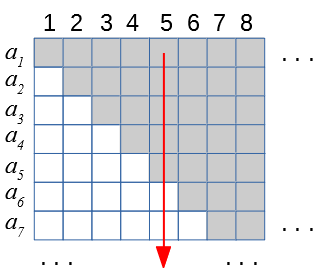
\includegraphics[width=2in]{prime-gaps.png}

Kā redzams šajā attēlā, katrā rindiņā arvien garāks sākumfragments ir nokrāsots balts (tur pirmskaitļu nevar būt, 
jo faktoriāla summu ar attiecīgo skaitli vienmēr var sadalīt reizinātājos).

Apskatāmies, vai saskaitot vienu un to pašu skaitli (teiksim, fiksētu skaitli $j = 5$) ar visiem virknes $a_1,a_2,a_3,\ldots$ 
locekļiem) iegūstam saliktus skaitļus vai pirmskaitļus? 
Tas nozīmē virzīšanos pa kolonnu (sarkanā bulta zīmējumā). No attēla redzams, ka dažas pirmās vērtības $a_k + 5$ 
(mūsu gadījumā tieši piecas) ir pelēkas: nezinām, vai tās ir pirmskaitļi vai nē. 
Virzoties pa šo kolonnu vēl zemāk, iegūsim tikai saliktus skaitļus, jo visi $k! + 1 + 5 = k! +6$ 
pietiekami lieliem $k$ dalīsies ar $6$ (tātad nebūs pirmskaitļi). Līdzīgi var spriest jebkurai 
citai vertikālei šajā tabulā \textendash{} pelēkā krāsā būs tikai galīgs skaits rūtiņu. $\blacksquare$

\vspace{5pt}
{\em Piezīme.} Kaut arī visi pirmskaitļi, sākot ar $a_1+1$, parādās divdimensiju tabulas rūtiņās (varbūt pat vairākās vietās)
un dažādo pirmskaitļu ir bezgalīgi daudz \textendash{} tomēr katrā tabulas vertikālē pirmskaitļu ir tikai galīgs skaits.





\newpage
{\bf Uzdevums 1.4.}\\
Par šādu apakšvirkni izvēlamies 
$$S = \left\{ \underbrace{11}_2,\;\underbrace{111}_3,\; \underbrace{11111}_5,\; \underbrace{1111111}_7,\; \underbrace{11111111111}_{11},\ldots \right\}.$$
Šajā virknē ietilpst visi tie skaitļi, kuru decimālpierakstā ir $p$ vieninieki (kur $p$ ir jebkurš pirmskaitlis).

\vspace{5pt}
{\em Pierādījums.} Jāpārbauda, ka jebkuri divi šīs virknes elementi ir savstarpēji pirmskaitļi. 
Lai to pārbaudītu, darbināsim Eiklīda algoritmu skaitļiem, kuru pierakstu veido attiecīgi $p_1$ un $p_2$ vieninieki, 
kur $p_1, p_2$ ir divi dažādi pirmskaitļi ($p_1 > p_2$). Izrādās, ka atlikums no dalījuma būs skaitlis, kuru veido 
$r$ vieninieki, kur $r$ ir atlikums $p_1$ dalot ar $p_2$. Piemēram,
\begin{equation}
\label{eq:multiones}
\mbox{LKD}\left(11111111111111111,1111111 \right) = \mbox{LKD}\left( 1111111, 111 \right) = \mbox{LKD}(111,1) =1.
\end{equation}

Piemēram, dalot skaitli ${\displaystyle \frac{10^{17}-1}{9}} = 11111111111111111$, kura pierakstā ir $17$ vieninieki 
ar skaitli $1111111$, kura pierakstā ir $7$ vieninieki, iegūsim atlikumu $111$, kurš sastāv no trim vieniniekiem.
(Jo, $17$ dalot ar $7$, rodas atlikums $3$.) Par to, ka šāds atlikums vienmēr rodas, var pārliecināties, izmantojot 
``skolas  algoritmu'' dalīšanai stabiņā. Vai ar sekojošām vienādībām (kur labajā pusē pirmie divi d
$$\frac{11111111111111111}{1111111} = \frac{11111110000000000  + 1111111000 + 111}{1111111} = 10000000000 + 1000 + \frac{111}{1111111}.$$

Līdzīgi arī jebkuriem citiem  skaitļiem, kuru pierakstā ir tikai vieninieki, var viegli veikt dalīšanas darbības un atrast atlikumu.
Tāpēc, ja sākam ar jebkuriem diviem skaitļiem no virknes $S$, tad to lielākā kopīgā dalītāja (LKD) meklēšana
būs līdzīga LKD meklēšanai starp diviem pirmskaitļiem \textendash{} abos gadījumos rezultāts būs $1$. 
Teiksim, vienādojumam (\ref{eq:multiones}) atbilstošais pirmskaitļu LKD meklēšanas algoritmms ir dots vienādojumā (\ref{eq:primes}): 
\begin{equation}
\label{eq:primes}
\mbox{LKD}\left(17,7 \right) = \mbox{LKD}(7,3) = \mbox{LKD}(3,1) = 1.
\end{equation}

Eiklīda algoritms (gan pašiem pirmskaitļiem, gan arī vieninieku virknēm) arvien dos rezultātu $1$, t.i.\
katri divi skaitļi no $S$ būs savstarpēji pirmskaitļi. $\blacksquare$



\newpage
{\bf Uzdevums 1.5.} Atbilde: Abi apgalvojumi ir aplami.

\vspace{10pt}
{\bf (A)} Formulēsim noliegumu šajā punktā dotajam apgalvojumam:
{\em ``Eksistē $k \geq 2$, un tādi $k$ pēc kārtas sekojoši skaitļi, starp kuriem 
visi dalās ar kādu no pirmskaitļiem, kas mazāks par $k$.''}\\
Izvēlamies $k=8$ un astoņus pēc kārtas sekojošus skaitļus $\{ 2,3,4,5,6,7,8,9 \}$. 
Katrs no tiem dalās ar kādu pirmskaitli $2,3,5,7$ (kas visi mazāki par $k=8$). 

\vspace{10pt}
{\bf (B)} Ir iespējams atrast $k = 17$ pēc kārtas sekojošus
naturālus skaitļus no $N$ līdz $N+16$, no kuriem ikviens dalās ar kādu pirmskaitli no $2$ līdz $13$. Un arī ikvienam
no šiem $17$ skaitļiem ir kāds kopīgs dalītājs (lielāks par $1$) ar kādu citu skaitli no šīs virknes.
Konstrukciju veicam, atzīmējot atsevišķās rindās ar bumbulīšiem skaitļus, kuri dalās attiecīgi
ar $2$, $3$, $5$, $7$, $11$ un $13$. Bumbulīšu rindas sabīdām tā, lai
vismaz viens bumbulītis atrastos katrā kolonnā; un vienlaikus - katrā rindā būtu vismaz divi bumbulīši,
t.i. būtu redzami skaitļi, kuri nav savstarpēji pirmskaitļi, jo tiem ir kopīgs dalītājs, kas lielāks par $1$.

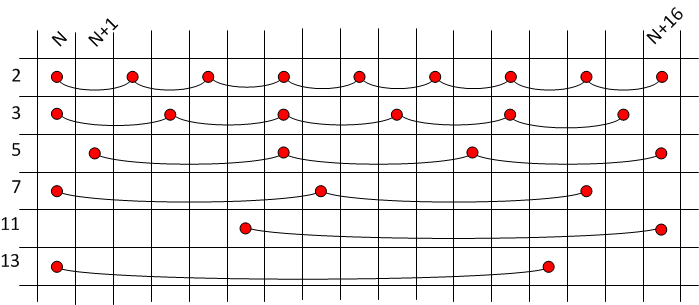
\includegraphics[width=4in]{bw2016-2.png}

Vēl jānoskaidro jautājums, vai $N$ var atrast tā, lai rastos visi zīmējumā redzamie atlikumi
ar pirmskaitļiem no $2$ līdz $13$ jeb mums vajadzīgās ``sākumfāzes''. Citiem vārdiem, vai eksistē tāds
naturāls $N$, kas dalās ar $2,3,7,13$ bez atlikuma un 
arī dod atlikumu $4$, dalot ar $5$, bet atlikumu $6$, dalot ar $11$. 
Šos daudzos atlikumus varam pierakstīt, izmantojot {\em kongruenču apzīmējumus}:
vajag, lai vienlaicīgi izpildās sešas kongruences:

\[
\left\{
\begin{array}{cccl}
N & \equiv & 0 & (\operatorname{mod}\,2) \\
N & \equiv & 0 & (\operatorname{mod}\,3) \\
N & \equiv & 4 & (\operatorname{mod}\,5) \\
N & \equiv & 0 & (\operatorname{mod}\,7) \\
N & \equiv & 6 & (\operatorname{mod}\,11) \\
N & \equiv & 0 & (\operatorname{mod}\,13)
\end{array}
\right.
\]

Tā kā moduļi ir pēc skaitļiem $2, 3, 5, 7, 11, 13$ (kas ir savstarpēji pirmskaitļi), šai 
kongruenču sistēmai vienmēr eksistē atrisinājums (tā ir {\em Ķīniešu atlikumu teorēma}).
Pirmā, otrā, ceturtā un sestā kongruence izpildās, ja vien $N = 2 \cdot 3 \cdot 7 \cdot 13 \cdot k$ kādam
naturālam $k$. Izvēloties $k = 4$, izpildās arī atlikušās divas kongruences. Tātad
$N = 2184$ un $17$ pēc kārtas sekojošie skaitļi ir, piemēram, šādi:
\[ \{ 2184, 2185, 2186, \ldots, 2198, 2199, 2200 \}. \]

\vspace{5pt}
{\em Piezīme 1.} Atrastā vērtība $N=2184$ nav vienīgā. Pēc Ķīniešu atlikumu teorēmas, der arī 
skaitļi $N=2184 + 30030\ell$, kur $\ell$ ir vesels skaitlis, bet $30030 = 2 \cdot 3 \cdot 5 \cdot 7 \cdot 11 \cdot 13$. 

\vspace{5pt}
{\em Piezīme 2.} Piemērs ar skaitļu intervālu $[2184;2200]$ un citiem līdzīgiem parāda, ka Eratostēna 
režģī mēdz rasties gari gabali, kuros nav neviena pirmskaitļa \textendash{} turklāt visi saliktie skaitļi 
tur dalās ar salīdzinoši nelieliem pirmskaitļiem (mūsu gadījumā no $2$ līdz $13$). 

\newpage

{\bf Uzdevumu avoti}

\begin{enumerate}
\item T.Andreescu et. al. {\em 104 Number Theory Problems.} Birkhäuser, 2007. (p.83. p.133). 
Sk. \url{https://bit.ly/3oUGw0y}.
\item T.Andreescu et. al. {\em 104 Number Theory Problems.} Birkhäuser, 2007. (p.84. p.138). 
Kā avots tur norādīta Pēterburgas olimpiāde (St.Petersburg, 2001), bet 2001.g. komplektā šāda uzdevuma nebija.
\item T.Andreescu et. al. {\em 104 Number Theory Problems.} Birkhäuser, 2007. (p.84. p.139). 
\item T.Andreescu et. al. {\em 104 Number Theory Problems.} Birkhäuser, 2007. (p.85. p.144). 
Kā avots tur norādīta Mathematical Olympiad Summer Program \textendash{} ASV olimpiāžu gatavošanas 
vasaras nometne (MOSP, 1997), bet šo komplektu neizdevās atrast.
\item Baltic Way, 2016, 2.uzdevums. Sk. \url{https://bit.ly/31Zqxo1}. Arī \url{https://bit.ly/37XJ9bK} un 
\url{https://bit.ly/2GfqAV0}.
\end{enumerate}


\end{document}